\begin{frame}[t]{Datenanalyse}
	\begin{block}{Convolutional Neural Network}
		\only<1>{
			\vspace{0.4cm}
			\begin{columns}[onlytextwidth]
				\begin{column}{0.45\textwidth}
					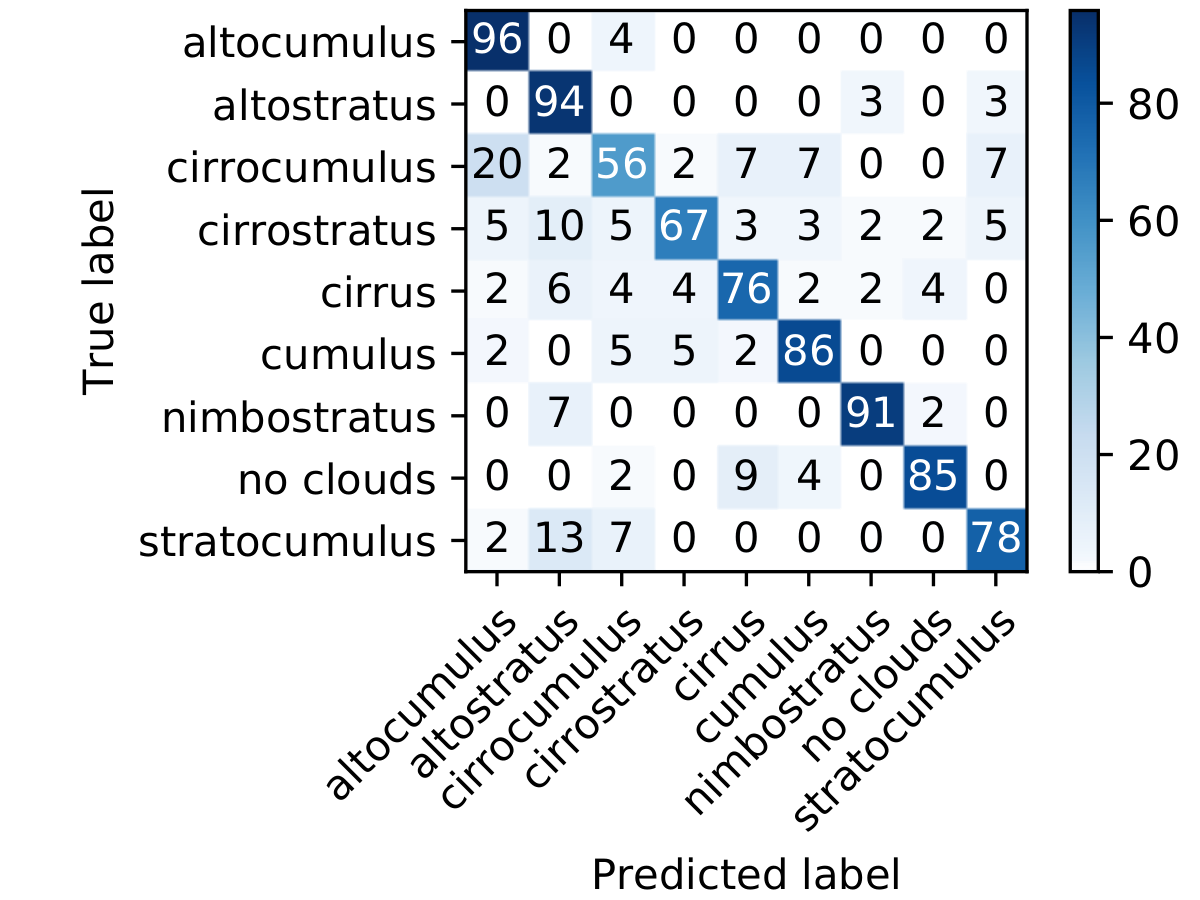
\includegraphics[width=\linewidth]{picture/conf_nn.png}
				\end{column}
				\begin{column}{0.55\textwidth}
					\centering
					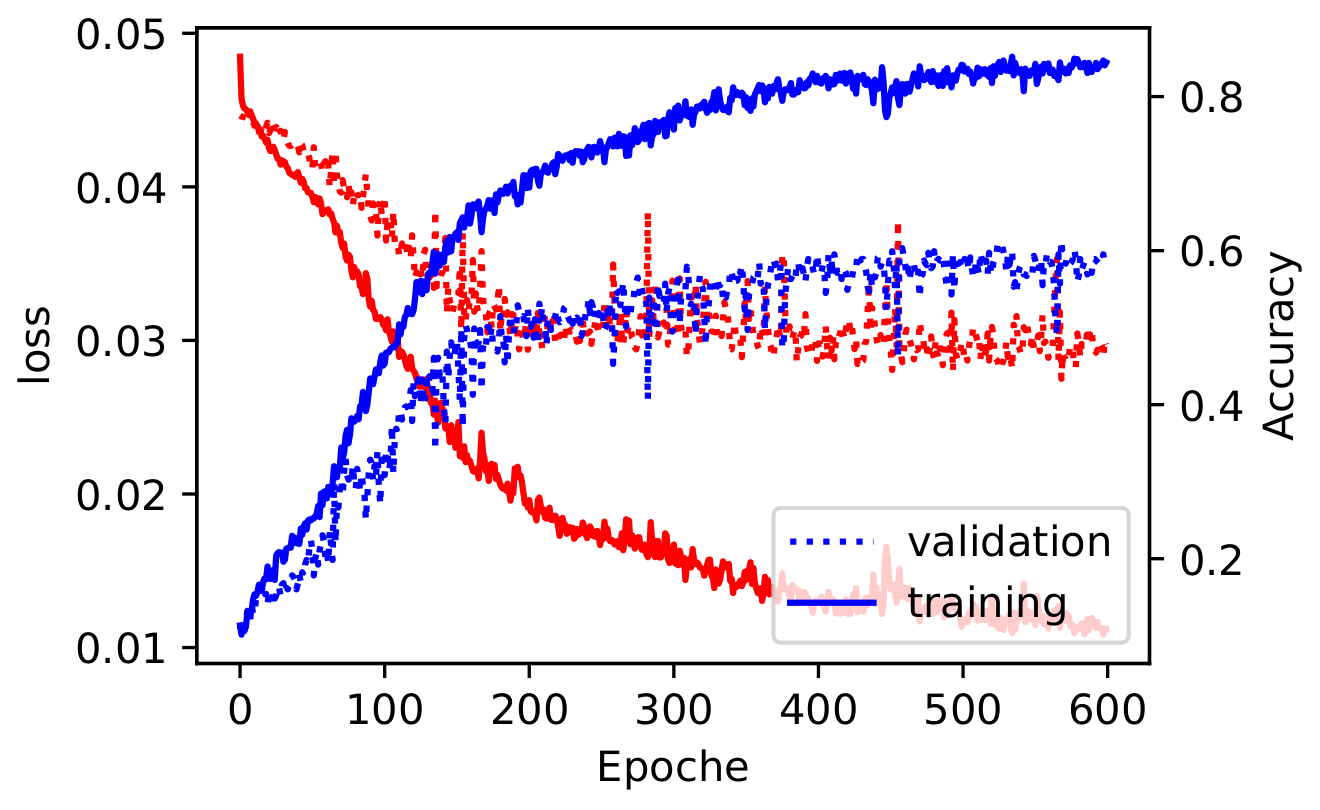
\includegraphics[width=0.8\linewidth]{picture/train_nn.png}
				\end{column}
			\end{columns}
			\vspace{0.2cm}
		}
		\only<2>{
			Klassifizierung der Wolkenfotos in 9 Klassen.
		}
	\end{block}
	\begin{block}{Farbschnitte}
		\only<1>{
			Farbschnitte auf den Kan\"alen der Bilder
		}
		\only<2>{
			\centering
			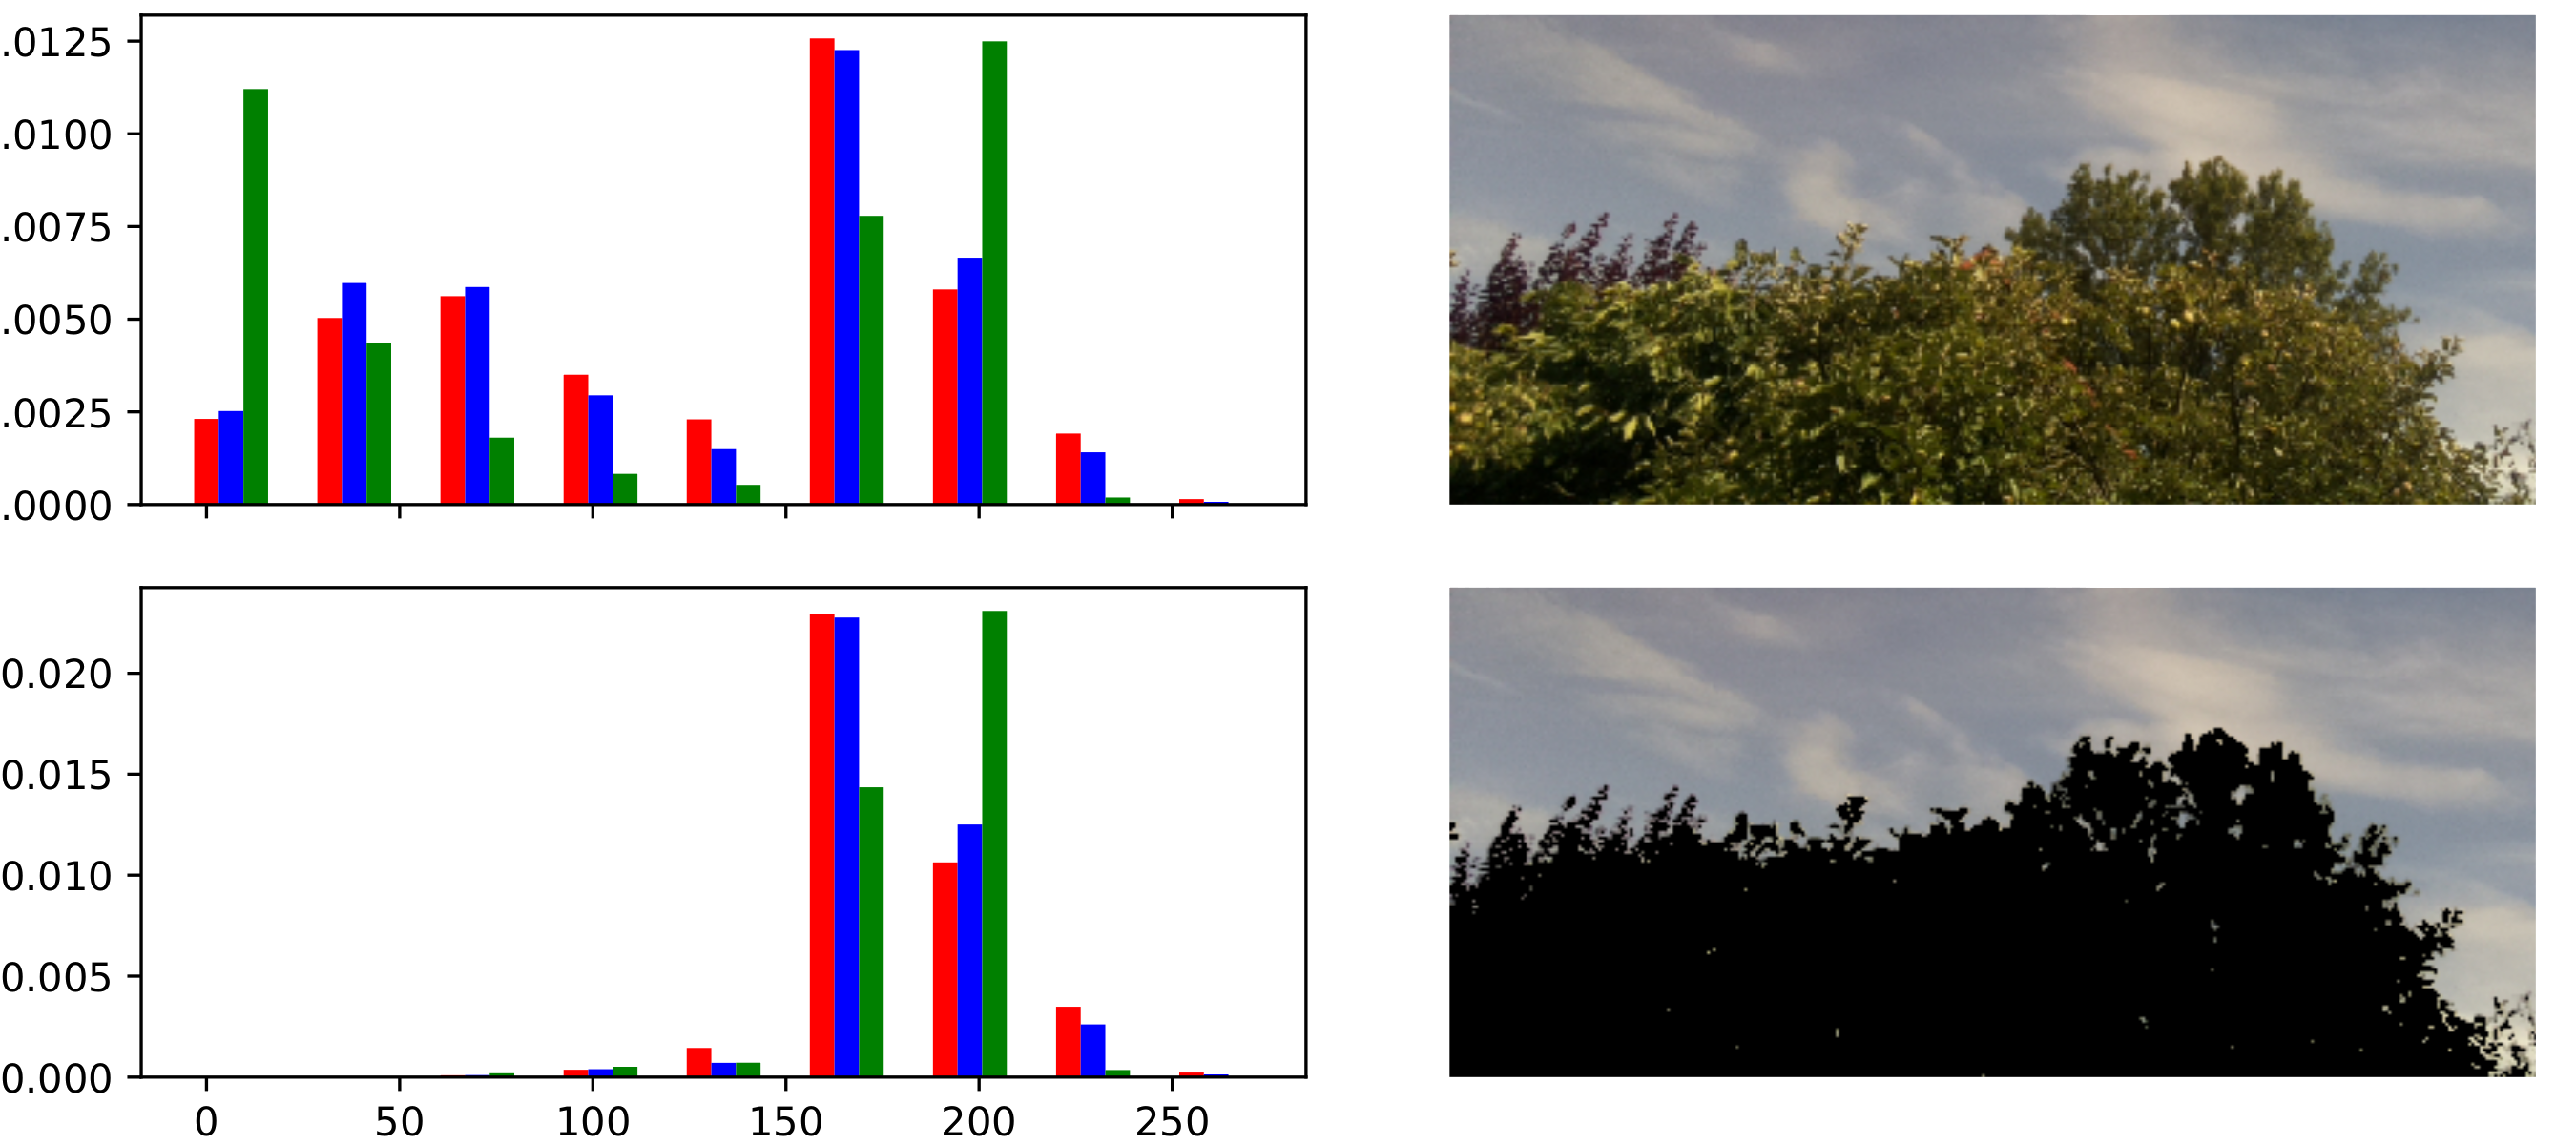
\includegraphics[width=0.95\linewidth]{picture/cut_hist.png}
		}
	\end{block}
\end{frame}
